% ME3050 -  Dynamics Modeling and Controls - Tennessee Technological University
% Tristan Hill - Spring 2020 - Summer 2020 - Spring 2022
% Dynamics Modeling and Controls
% Lecture Module - Dynamics Review  - Topic 2  - Coordinate Systems 

% Document settings

%\documentclass{beamer}                  % for presentation ?
\documentclass[handout]{beamer}  % for handout ?

\usepackage{/home/thill/Documents/lectures/dmc_lectures/dmc_lectures}

\newcommand{\MNUM}{2\hspace{2mm}} % Module number
\newcommand{\TNUM}{2\hspace{2mm}} % Topic number 
\newcommand{\moduletitle}{Dynamics Review} % Titles and Stuff
\newcommand{\topictitle}{Coordinate Systems} 

\newcommand{\sectiontitleI}{Using Different Coordinate Systems} % More Titles and Stuff
\newcommand{\sectiontitleII}{Cartesian}
\newcommand{\sectiontitleIII}{Polar and Cylindrical}
\newcommand{\sectiontitleIV}{Spherical}
\newcommand{\sectiontitleV}{Others ?}



\author{ME3050 - Dynamic Modeling and Controls}
\title{Lecture Module - \moduletitle}
\date{Mechanical Engineering\vspc Tennessee Technological University}

\begin{document}
	
	\lstset{language=MATLAB,basicstyle=\ttfamily\small,showstringspaces=false}
	
	\frame{\titlepage \center\begin{framed}\Large \textbf{Topic \TNUM - \topictitle}\end{framed} \vspace{5mm}}
	
	% Section 0 - Outline
	\frame{
		
		\large \textbf{Topic \TNUM - \topictitle} \vspace{3mm}\\
		
		\begin{itemize}
			
			\item \sectiontitleI    \vspc % Section I
			\item \sectiontitleII 	\vspc % Section II
			\item \sectiontitleIII 	\vspc %Section III
			\item \sectiontitleIV 	\vspc %Section IV
			%\item \sectiontitleV 	\vspc %Section V
			
		\end{itemize}
		
	}
	
	

% Section 1:
\section{Using Different Coordinate Systems}

\frame{
\frametitle{Using Different Coordinate Systems}

It is often convienent to use different coordinate systems as a reference for different types of problems. \vspc

You, the engineer and designer must choose the coordinate system.

}

% Section 2: 
\section{Cartesian}

\frame{
\frametitle{Cartesian}

The \href{https://en.wikipedia.org/wiki/Cartesian_coordinate_system}{Cartesian Coordinate System} 


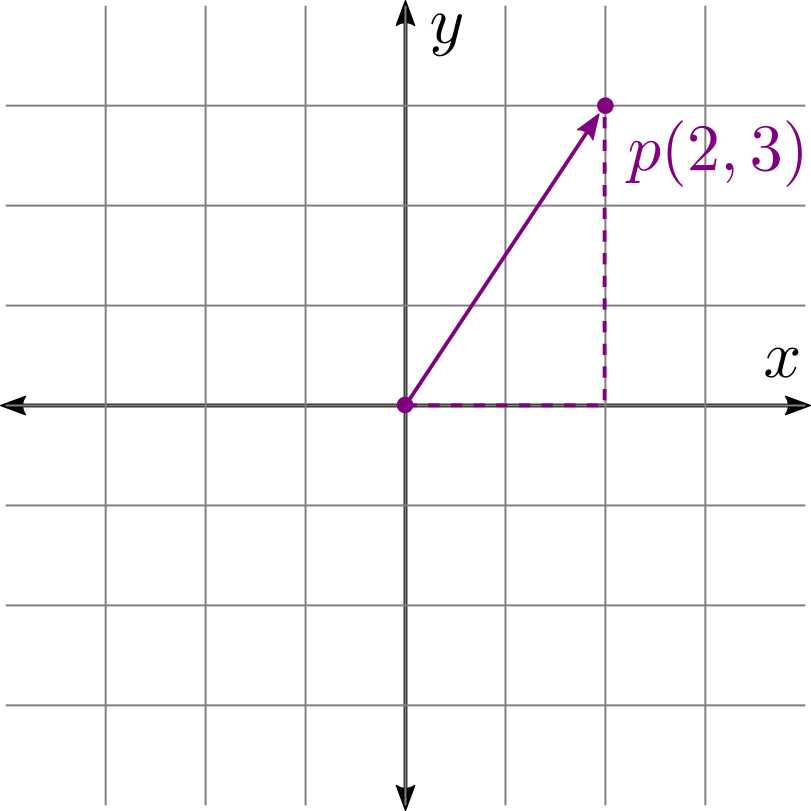
\includegraphics[scale=.175]{cartesian.png} \hspccc \hspccc
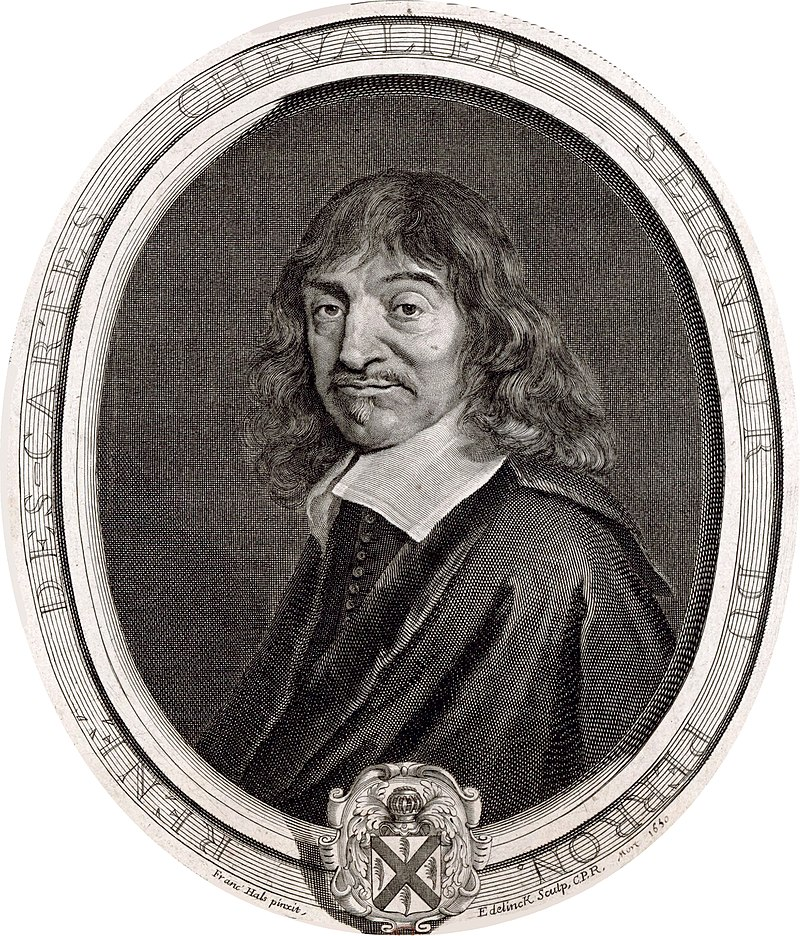
\includegraphics[scale=.125]{Descartes.jpg} \\ \hspace{80mm} {\tiny \href{https://en.wikipedia.org/wiki/Ren\%C3\%A9_Descartes}{Image: Wikipedia} }

}

\frame{
\frametitle{Rotated Cartesian}

It is common to use a Cartesian coordinate system that has been rotated such that it is aligned with a particular problem. 

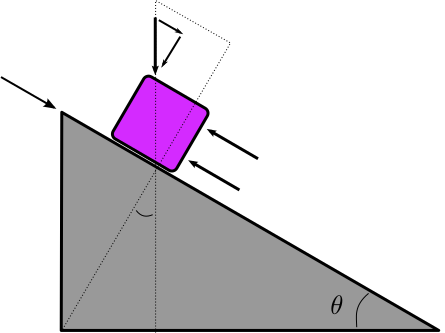
\includegraphics[scale=.4]{sliding_block.png}

}


% Section 3: 
\section{Polar and Cylindrical}

\frame{
\frametitle{Polar and Cylindrical}

For problems involving rotation it is convient to use polar or cylindrical coordinate systems. Conversion from Cartesian to polar  is straightforward using trigonometry. 

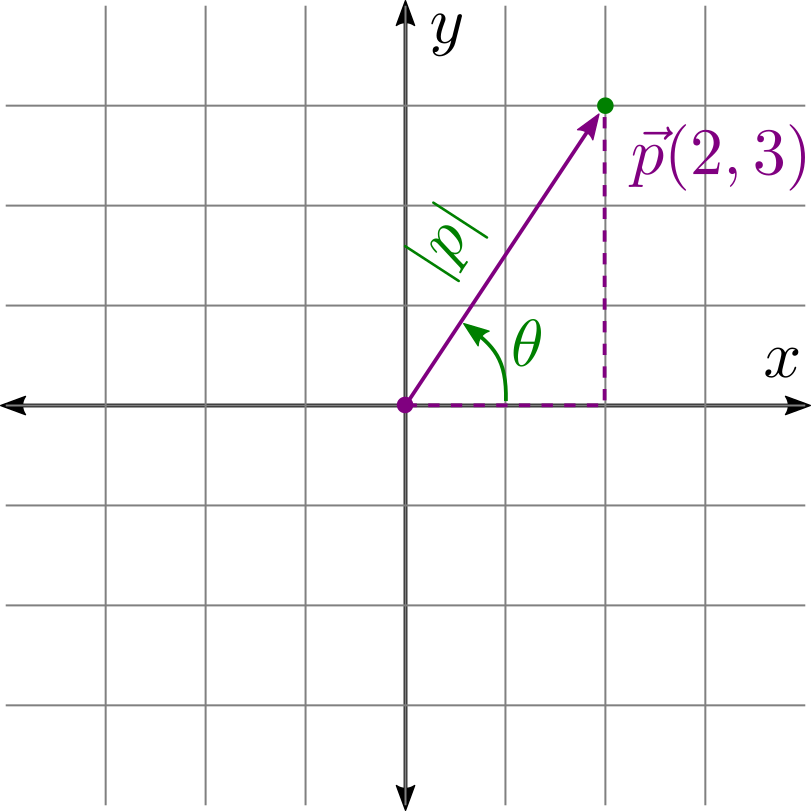
\includegraphics[scale=.18]{polar.png} \hspccc \hspccc 
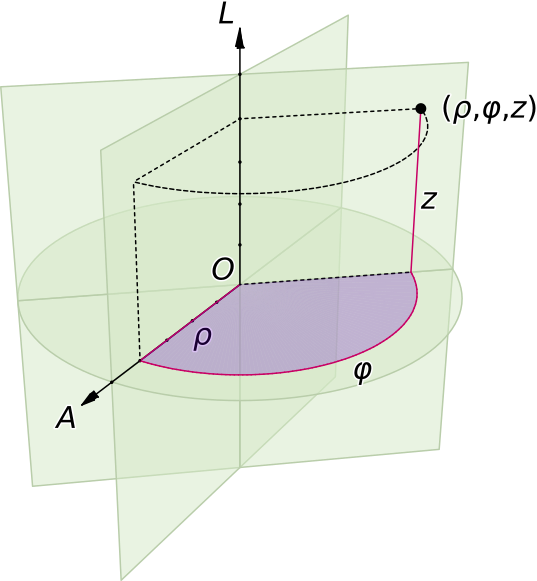
\includegraphics[scale=.275]{cylindrical.png}\\ \hspace{80mm} {\tiny \href{https://en.wikipedia.org/wiki/Cylindrical_coordinate_system}{Image: Wikipedia} }

}

% Section 4:
\section{Spherical}

\frame{
\frametitle{Spherical}

``The spherical coordinate system generalizes the two-dimensional polar coordinate system...'' {\tiny \href{https://en.wikipedia.org/wiki/Spherical_coordinate_system}{Wikipedia} }

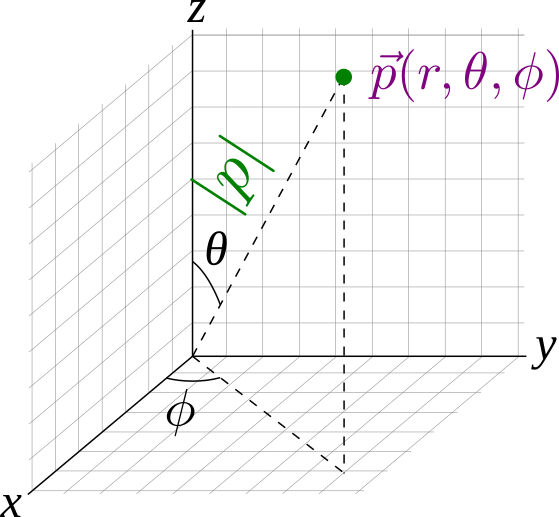
\includegraphics[scale=.3]{spherical_fig1.png} \hspccc \hspccc
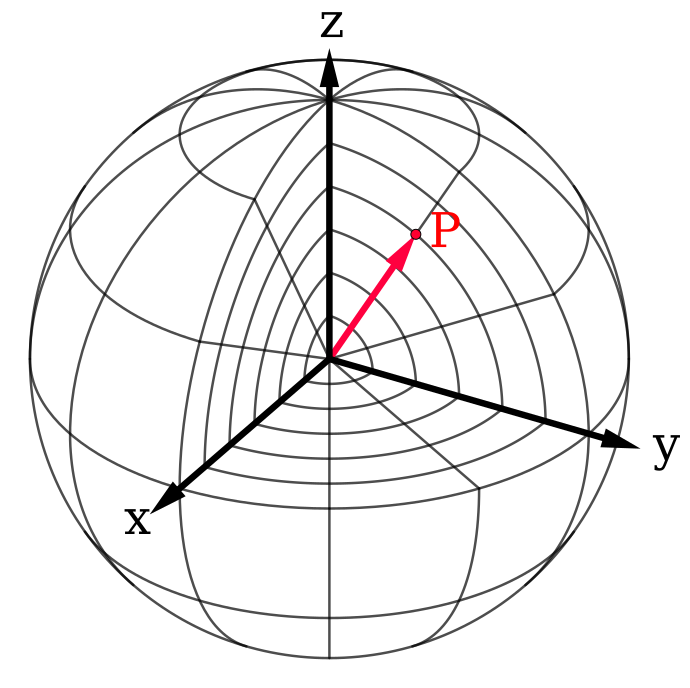
\includegraphics[scale=.2]{spherical_fig2.png}  \\ {\tiny \href{https://en.wikipedia.org/wiki/Spherical_coordinate_system}{Image: Wikipedia} } \hspace{60mm} {\tiny \href{https://en.wikipedia.org/wiki/Spherical_coordinate_system}{Image: Wikipedia} }


}

% Section 5:
\section{Others ?}

\frame{
\frametitle{Others ?}

Do you know of any other systems that are used?

}
	
\end{document}



